\chapter{Altri es. MR}
\section{Es.1 - tavolo cliente}
\subsubsection{Specifiche}
Il seguente schema relazionale riguarda un sistema di prenotazione e gestione dei tavoli di un ristorante. Il sistema in fase di prenotazione prevede una fase di registrazione in cui il cliente deve immettere i propri dati tra cui il codice fiscale, nome, cognome, e altro. Ogni tavolo ha un codice identificativo e numero di coperti massimo. Una prenotazione può riferirsi al turno pranzo o cena. Un tavolo può essere utilizzato solo una volta durante un turno. Un addetto del ristorante può servire più tavoli ma ogni tavolo è servito da un solo addetto. Ogni tavolo è dotato di un tablet attraverso cui è possibile sfogliare il menu e ordinare i pasti. Il tablet viene fornito dall'addetto al servizio al cliente ad inizio pranzo o cena. I tavoli sono disposti in diverse sale separate che possono essere 'normali' o sale in cui si proiettano eventi sportivi e concerti.

\subsubsection{Relazioni}
TABLET (codice, marca, modello, dataAcquisto, scadenzaGaranzia)
\\TAVOLO (codice, numeroCoperti, sala)
\\CLIENTE (codiceFiscale, nome, cognome, indirizzo, cap, citta, numTel, email)
\\GESTIONETAVOLO (codiceTavolo, cliente, data, turno, addettoRistorante, tablet)
\\PERSONALERISTORANTE (codiceFiscale, nome, cognome, stipendio, annoNascita, annoAssunzione)
\\SALA (codice, tipologia)

\subsubsection{Chiavi primarie}
TABLET (\underline{codice}, marca, modello, dataAcquisto, scadenzaGaranzia)
\\TAVOLO (\underline{codice}, numeroCoperti,sala)
\\CLIENTE (\underline{codiceFiscale}, nome, cognome, indirizzo, cap, citta, numTel, \underline{email})
\\GESTIONETAVOLO (\underline{codiceTavolo}, cliente, \underline{data}, \underline{turno}, addettoRistorante, tablet)
\\PERSONALERISTORANTE (\underline{codiceFiscale}, nome, cognome, stipendio, annoNascita, annoAssunzione)
\\SALA (\underline{codice}, tipologia)

\subsubsection{Chiavi esterne}
\begin{center}
    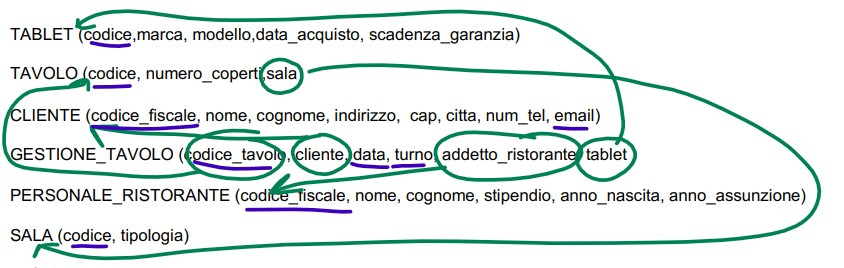
\includegraphics[width=0.675\textwidth]{chaptersLezioniSara/img/MR_altrofile_es1.jpg}
\end{center}

\subsubsection{Vincoli di tupla}
data.acquisto < scadenza + 2
\\anno-nascita $\leq$ anno-assunzione + 18
\\CAP = seq numeri interi L = 5
\\numero-coperti > 0

\section{Es.2 - gestione magazzino}
\subsubsection{Specifiche}
Il seguente schema relazionale riguarda un sistema per la gestione di una palestra. In palestra possono entrare solo gli iscritti con abbonamento in corso di validità. All'entrata gli iscritti utilizzano un badge che permette di aprire il tornello di entrata solo se l'abbonamento è in corso di validità. Gli abbonamenti possono essere di diversa tipologia: mezza giornata, giornata piena ecc.. La palestra è composta da sale ognuna destinata ad una tipologia di attività: attrezzi, corpo libero ecc. In una data sala viene svolta una specifica attività e opera un solo addetto. Nelle sale possono esserci degli attrezzi. Dalla palestra vengono offerte gratuitamente (incluso nell'abbonamento) delle lezioni di gruppo come «lezione di aerobica», «zumba» ecc. che sono svolte in un dato giorno e ora della settimana in una data sala sempre dallo stesso addetto.

\subsubsection{Relazioni}
ATTREZZATURA (codice, marca, modello, dataAcquisto, scadenzaGaranzia, sala)
\\LEZIONE (codiceLezione, nome, giorno, ora, sala, addetto)
\\ISCRITTO (codiceFiscale, nome, cognome, indirizzo, cap, citta, numTel, email)
\\ABBONAMENTO(iscritto, dataInizio, dataFine, tipologia)
\\ADDETTO (codiceFiscale, nome, cognome, stipendio, annoNascita, annoAssunzione)
\\SALA (codice, tipologiaAttività, addetto)

\subsubsection{Chiavi primarie}
ATTREZZATURA (codice, marca, modello, dataAcquisto, scadenzaGaranzia, sala)
\\LEZIONE (codiceLezione, nome, giorno, ora, sala, addetto)
\\ISCRITTO (codiceFiscale, nome, cognome, indirizzo, cap, citta, numTel, email)
\\ABBONAMENTO(iscritto, dataInizio, dataFine, tipologia)
\\ADDETTO (codiceFiscale, nome, cognome, stipendio, annoNascita, annoAssunzione)
\\SALA (codice, tipologiaAttività, addetto)

\subsubsection{Vincoli di tupla}
data acquisto < scadenza garanzia
\\data inizio < data fine
\\anno nascita $\leq$ anno assunzione 

\section{Es.3 - libreria}
\subsubsection{Specifiche}
Lo schema seguente rappresenta una base di dati impiegata in una catena di librerie distribuite su tutto il territorio nazionale. In particolare, oltre ai dati sulle singole librerie, sono archiviati i dati del personale e dei libri in vendita. Si osservi che possono esistere diverse versioni dello stesso libro (autore e titolo), edite da case editrici diverse. Infine, attraverso la relazione Catalogo è possibile conoscere in quali librerie una determinata versione di un libro sia disponibile per essere venduta, il numero di copie a disposizione, ed il costo. 

\subsubsection{Relazioni}
LIBRERIA(idLibreria, indirizzo, città, oraApertura, oraChiusura, turnoChiusura)
\\PERSONALE(idPersona, cognome, nome, idLibreria, reparto, turno)
\\CATALOGO(idLibro, idLibreria, reparto, numerocopie, costo)
\\LIBRO(idLibro, titolo, autori, casaEditrice, annoPubblicazione)

\subsubsection{Chiavi primarie}
LIBRERIA(\underline{idLibreria}, indirizzo, città, oraApertura, oraChiusura, turnoChiusura)
\\PERSONALE(\underline{idPersona}, cognome, nome, idLibreria, reparto, turno)
\\CATALOGO(\underline{idLibro}, \underline{idLibreria}, reparto, numerocopie, costo)
\\LIBRO(\underline{idLibro}, titolo, autori, casaEditrice, annoPubblicazione)

Chiavi alternative:
\\"indirizzo" e "città" per Libreria.

Possibile superchiave:
\\tutta la tupla di una qualsiasi relzione, es la riga di Libro.

\subsubsection{Vincoli di ennupla}
orario apertura < orario chiusura

\subsubsection{Vincoli di dominio}
costo > 0
\\numerocopie $\geq$ 0
\\turnoChiusura $\in$ {lunedi, martedi, mercoledi, giovedi, venerdi, sabato, domenica}